% Progress report: max 3 pages excluding references, single column.
% Short version of report.tex; every number here is the same as in report.tex.
\documentclass[11pt]{article}

\usepackage[margin=1in]{geometry}
\usepackage[T1]{fontenc}
\usepackage[utf8]{inputenc}
\usepackage{lmodern}
\usepackage{amsmath}
\usepackage{booktabs}
\usepackage{tabularx}
\usepackage{graphicx}
\usepackage{enumitem}
\usepackage{tikz}
\usetikzlibrary{positioning,arrows.meta}
\usepackage[numbers,sort&compress]{natbib}
\usepackage[hidelinks]{hyperref}
\usepackage{xurl}

\setlist{nosep,leftmargin=*}
\setlength{\parskip}{0.3em}
\setlength{\parindent}{0pt}

\title{\vspace{-2.4em}\textbf{DGA Classifier from Domain Names: Family-First or Direct Binary?}\\[0.2em]\large Progress Report}
\author{
  Roudy Barakat \quad \texttt{rtb07@mail.aub.edu} \qquad
  Abdo Sebaali \quad \texttt{ams86@mail.aub.edu} \\[0.2em]
  \small American University of Beirut, EECE 690
}
\date{\vspace{-2.2em}}

\begin{document}
\maketitle

\section{Refined Problem and Dataset}
Malware uses domain generation algorithms (DGAs) to reach its servers through
thousands of throw-away domains~\cite{plohmann2016dgarchive}, so a DNS filter must
recognise generated names from the name alone. Some families produce random
strings (\texttt{gqspwpsurdun.ru}) or hex hashes, others join dictionary words
(\texttt{kneemanualgirl.com}) and look legitimate.

\textbf{Question.} For a DGA/legitimate decision, is it better to train on the DGA
families and collapse the prediction (\emph{family-first}), or to train on the
binary label directly (\emph{binary})? For each model we measure
$\Delta = \text{macro-F1}_{\text{family-first}} - \text{macro-F1}_{\text{binary}}$
on the same evaluation set, with everything but the training labels held fixed.
Family-first counts as better if $\Delta > 0$ by more than its uncertainty.

\textbf{Dataset.} 1{,}999{,}335 domains: 999{,}664 legitimate from the Tranco top
1M~\cite{lepochat2019tranco} and 999{,}671 DGA in 103 families, from
DGArchive via Greg{\'o}rio and Cansian~\cite{gregorio2025dataset,plohmann2016dgarchive}
and Kaggle~\cite{givre2021kaggle}. We removed 330 domains found in both lists,
141 duplicates and 7 invalid strings; merged the 59 families under 300 domains into
\texttt{other\_dga}; and capped each family at 29{,}120 so that DGA and legitimate
are equal in number. Sample weights give each class half the weight and, within
DGA, are proportional to $1/\sqrt{n_f}$ ($n_f$: family size). One fixed 80/10/10
split, stratified by family~\cite{shahzad2021dga}, is shared by every model:
1.6M training, 200k validation and 200k test domains. All results below are on
the validation set; the test set is kept for the final runs.

\section{Technical Approach}
Every model sees only the domain string and gives class probabilities
$p(\cdot \mid x)$ over 2 classes (binary) or 104 (\texttt{legit} + 103 families,
family-first). Both are turned into one DGA score $s(x)$, and a domain is called
DGA when $s(x) \ge 0.5$ in both setups (Fig.~\ref{fig:pipeline}). Family-first
adds up the probabilities of all families, $s(x) = 1 - p(\texttt{legit} \mid x)$,
so a domain the model believes is a DGA of an unknown family is still flagged.

\begin{figure}[h]
\centering
\resizebox{\linewidth}{!}{%
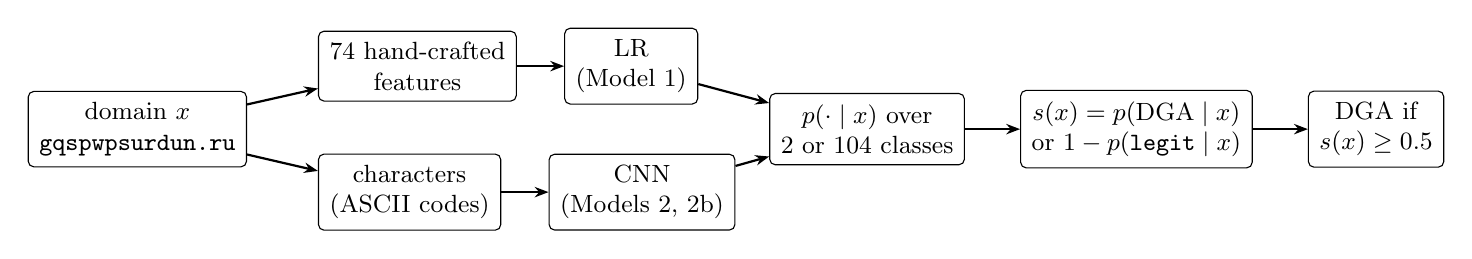
\begin{tikzpicture}[
  box/.style={draw, rounded corners=2pt, align=center, font=\small, inner sep=4pt, minimum height=2.2em},
  arr/.style={-{Stealth[length=5pt]}, thick}]
\node[box] (x) {domain $x$\\ \texttt{gqspwpsurdun.ru}};
\node[box, right=0.9cm of x, yshift=0.8cm] (f) {74 hand-crafted\\features};
\node[box, right=0.9cm of x, yshift=-0.8cm] (c) {characters\\(ASCII codes)};
\node[box, right=0.6cm of f] (lr) {LR\\(Model 1)};
\node[box, right=0.6cm of c] (cnn) {CNN\\(Models 2, 2b)};
\node[box, right=0.9cm of lr, yshift=-0.8cm] (p) {$p(\cdot\mid x)$ over\\2 or 104 classes};
\node[box, right=0.7cm of p] (s) {$s(x) = p(\text{DGA}\mid x)$\\or $1 - p(\texttt{legit}\mid x)$};
\node[box, right=0.7cm of s] (d) {DGA if\\$s(x) \ge 0.5$};
\draw[arr] (x) -- (f); \draw[arr] (x) -- (c);
\draw[arr] (f) -- (lr); \draw[arr] (c) -- (cnn);
\draw[arr] (lr) -- (p); \draw[arr] (cnn) -- (p);
\draw[arr] (p) -- (s); \draw[arr] (s) -- (d);
\end{tikzpicture}}
\caption{Pipeline. Only the training labels differ between the two setups: binary
($y$, 2 classes) or family-first ($z$, 104 classes).}
\label{fig:pipeline}
\end{figure}

\textbf{Model 1: logistic regression (LR) on hand-crafted features.} Each domain
is split by tldextract~\cite{kurkowski_tldextract} into name and suffix, and
described by 74 features: 7 basic (length, entropy, digit and hyphen ratios,
\dots), 7 n-gram scores, 2 Markov log-probabilities (orders 1 and 2), 4 vowel
features and 54 TLD features (one-hot of the 50 most common suffixes and 4
others). The n-gram and Markov counts are learned from legitimate training names
out-of-fold (10 folds), so no domain is scored with counts it helped build. LR
predicts $\operatorname{softmax}(xW + b)$ on the standardised features and
minimises the weighted cross-entropy with an L2 penalty
($\lambda = 10^{-4}$) by full-batch L-BFGS~\cite{liu1989lbfgs,virtanen2020scipy}
on the whole training set. We also test three variants: \emph{stacking}~\cite{wolpert1992stacked}
(out-of-fold family-first probabilities fed into a binary LR), and reducing the
features with \emph{PCA}~\cite{jolliffe2002pca} or \emph{LDA}~\cite{fisher1936lda}
to the number of components that keeps 95\% or 99\% of the variance.

\textbf{Model 2: reference CNN.} We re-run the character-level CNN of
\citet{gregorio2024incremental} in PyTorch~\cite{paszke2019pytorch}: an embedding
of the 93 padded ASCII codes, six convolutions with ReLU in three blocks, a
15-unit dense layer and an output of 2 or 104 units ($\approx$1.1M parameters).
It is trained with Adam~\cite{kingma2015adam} on the weighted cross-entropy plus
an elastic-net penalty~\cite{zou2005elasticnet}, for 40 epochs, keeping the epoch
with the highest validation macro-F1. Runs are tracked with
MLflow~\cite{zaharia2018mlflow}.

\textbf{Model 2b: revised CNN.} Inspecting Model 2 showed four weaknesses: its
output depends on where a pattern occurs, 6 of its 15 dense units never activate,
it overfits after about 10 epochs, and it reads the padding (83\% of the input)
as characters. Model 2b uses global max and mean pooling over the real
characters~\cite{kim2014cnn}, 128 filters and dense units, batch
normalisation~\cite{ioffe2015batchnorm} and dropout~\cite{srivastava2014dropout},
and masks the padding ($\approx$0.48M parameters); it is still training.

\section{Preliminary Results and What We Learned}
Table~\ref{tab:results} gives the results on the validation set, one run per setup.

\begin{table}[h]
\centering
\small
\caption{Validation results on the DGA/legitimate decision. $\Delta$:
family-first minus binary. A majority-class predictor reaches macro-F1 0.3333.}
\label{tab:results}
\begin{tabular}{@{}llcccc@{}}
\toprule
Model & Setup & Macro-F1 & DGA precision & DGA recall & ROC-AUC \\
\midrule
Model 1 (LR), with TLD & binary & 0.9212 & 0.9327 & 0.9079 & 0.9752 \\
 & family-first & 0.9397 & 0.9446 & 0.9342 & 0.9860 \\
 & $\Delta$ & $+0.0185$ & $+0.0119$ & $+0.0263$ & $+0.0108$ \\
LR, without TLD & binary & 0.9090 & 0.9227 & 0.8929 & 0.9588 \\
 & family-first & 0.9151 & 0.9319 & 0.8958 & 0.9641 \\
 & $\Delta$ & $+0.0061$ & $+0.0092$ & $+0.0029$ & $+0.0052$ \\
\midrule
LR + stacking, without TLD & binary & 0.9140 & 0.9420 & 0.8825 & 0.9622 \\
LR + PCA 95\%, with TLD & family-first & 0.9243 & 0.9301 & 0.9177 & 0.9796 \\
LR + LDA 95\%, with TLD & family-first & 0.9409 & 0.9464 & 0.9348 & 0.9861 \\
\midrule
Model 2 (reference CNN) & binary & 0.9747 & 0.9753 & 0.9739 & 0.9966 \\
 & family-first & 0.9751 & 0.9772 & 0.9729 & 0.9966 \\
 & $\Delta$ & $+0.0004$ & $+0.0019$ & $-0.0010$ & $0.0000$ \\
\midrule
Model 2b (revised CNN) & both & \multicolumn{4}{c}{\emph{pending: training in progress}} \\
\bottomrule
\end{tabular}
\end{table}

\textbf{What we learned.}
\begin{itemize}
  \item \emph{Family labels help the linear model:} for LR, family-first wins on
  every metric, by $+0.0185$ macro-F1 with the TLD and $+0.0061$ without. LR can
  draw only one boundary between legitimate names and all DGA families together;
  family-first gives it one boundary per family. The TLD makes the gain about
  three times larger, since many families use their own few suffixes.
  \item \emph{They barely change the CNN:} $\Delta = +0.0004$, with ROC-AUC equal
  at 0.9966. The CNN learns each family's patterns from the binary label alone,
  so the gain shrinks as the model gets more flexible. With one run per setup,
  $+0.0004$ cannot yet be told apart from run-to-run variation.
  \item \emph{The simple collapse is best:} stacking beats binary ($+0.0050$) but
  stays 0.0011 below plain family-first. PCA lowers macro-F1, since it ignores the
  labels; LDA, which uses them, matches all features with 55 of the 74 dimensions.
  \item \emph{The CNN overfits early:} its validation loss is lowest at epoch 9
  (binary) and 13 (family-first); Model 2b adds regularisation for this.
  \item \emph{Hard case:} dictionary DGAs such as matsnu and nymaim2 look
  legitimate to the name features and are mostly missed.
\end{itemize}

\section{Updated Plan and Risks}
\textbf{Plan.}
\begin{enumerate}
  \item Revised CNN (Model 2b) in both setups, compared with Model 2 (Nov 16--22).
  \item Uncertainty of $\Delta$: repeated seeds and a paired bootstrap on the
  saved predictions; both CNNs without the TLD; recall per family (Nov 23--29).
  \item Further models in both setups: an MLP on the 74 features, a convolutional
  autoencoder~\cite{masci2011cae}, a character-level
  Transformer~\cite{vaswani2017attention} for dictionary DGAs, and CNN embeddings
  joined with the hand-crafted features (Nov 23--29).
  \item One run of every final configuration on the test set; final report and
  presentation (Nov 30--Dec 6).
\end{enumerate}

\textbf{Risks.}
\begin{itemize}
  \item \emph{Small CNN gain:} $\Delta = +0.0004$ may be noise; the uncertainty
  estimate will decide.
  \item \emph{TLD shortcut:} 23 families use a single TLD, so the TLD alone
  separates them; we report every model with and without it.
  \item \emph{Data bias and validity:} Tranco favours popular sites, so unusual
  legitimate names may be flagged; we test only known families, and accuracy can
  drop on unseen ones~\cite{dahal2019autoencoded}.
  \item \emph{Compute time:} family-first training on 1.6M domains is slow (about
  25 minutes per LR fit, much longer per CNN), which limits the number of repeated runs.
\end{itemize}

\textbf{Code:} \url{https://github.com/RoudyBarakat/dga-detection}.

\bibliographystyle{plainnat}
\bibliography{refs}

\end{document}
